\chapter{Desktop Teleoperated Surgical Training System}

In an effort to further advance the field of robotic-assisted surgery, researchers at MCI have developed a Desktop Teleoperated Surgical Training System. The system's design was heavily inspired by the dVRK and Raven II, with a focus on maximizing performance while minimizing cost. This system serves as the foundation for the research outlined in this paper, so an understanding of its design and architecture is essential.

\section{Overall System Architecture}

The system consists of two main components, the MTM and the PSM.

While the system was conceptually designed to include both right and left MTMs and PSMs, the scope of this research was limited to a single-sided setup. Consequently, only one MTM and one PSM were manufactured and developed.

The MTM is a serial-link manipulator that measures the operator's motion and communicates it to the PSM, which replicates the movements at the surgical site. These individual systems will be explored further in the following sections, and an overview of the system can be seen in Figure~\ref{fig:system_overview}.

\begin{figure}[H] % Changed from [h] for better float placement
    \centering
    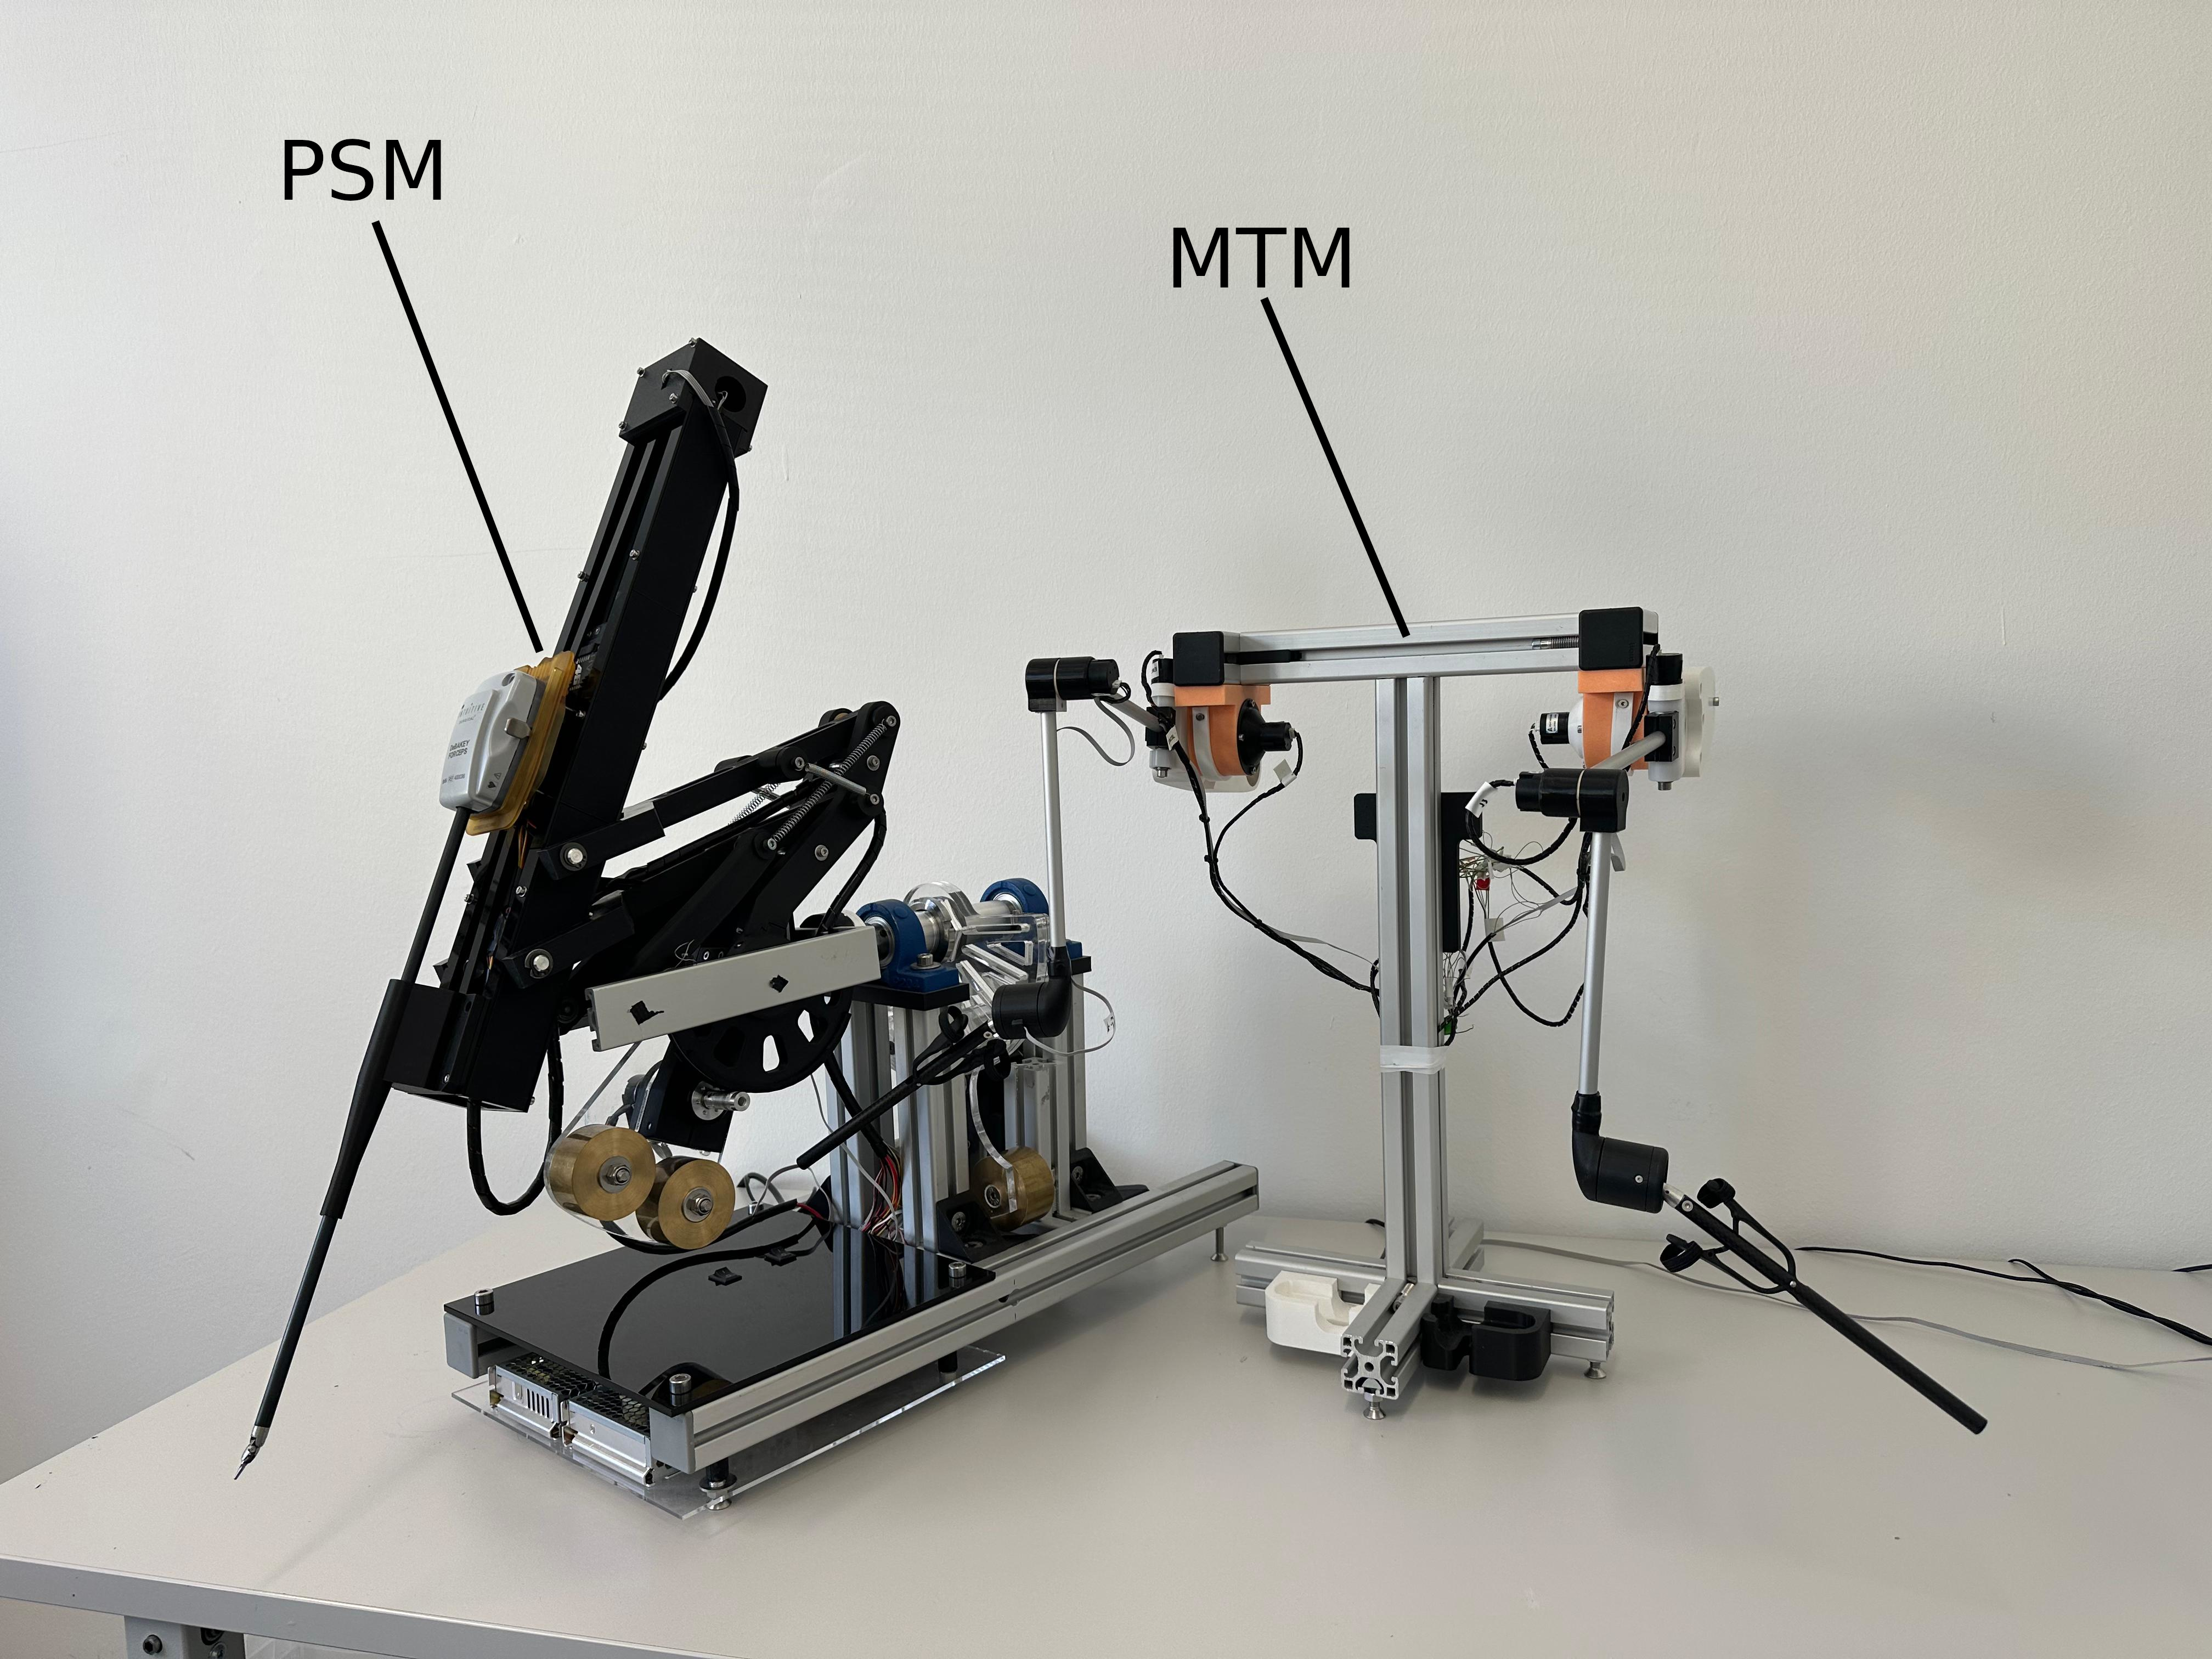
\includegraphics[width=.750\linewidth]{figures/system_overview.png}
    \caption{ Overview of the Desktop Teleoperated Surgical Training System, illustrating the MTM and PSM components.}
    \label{fig:system_overview} % Renamed label for consistency
\end{figure}


\subsection{MTM Overview}

The MTM is a serial-link manipulator that measures the operator's motion through a 7-DOF linkage, actuated by the user. The associated DOFs and their types are indicated in Table~\ref{tab:mtm_dofs_detailed}.

\begin{table}[H] 
    \caption{MTM Joint Classification and Positional Sensing.}
    \label{tab:mtm_dofs_detailed}
    \begin{tabular}{|l|l|l|}
    \hline
    \textbf{Joint Classification} & \textbf{Dof Name} & \textbf{Positional sensing} \\
    \hline
    \multirow{3}{*}{\raggedright Overall system positioning} & J0 & \multirow{3}{*}{12-bit absolute magnetic encoder} \\
    & J1 & \\
    & J2 & \\
    \hline
    \multirow{4}{*}{\raggedright Instrument positioning} & G0 & Hall Effect Sensor \\
    \cline{2-3}
    & G1 & \multirow{3}{*}{Analog Potentiometer} \\
    & G2 & \\
    & G3 & \\
    \hline
    \end{tabular}
\end{table}
These joints allow the operator to communicate desired motions to the PSM. The J0--J2 DOFs dictate the endpoint position, while G0--G3 control endpoint orientation and state.

The MTM should allow for accurate interpretation of the operator's intended motion while also minimizing the force perceived by the operator. This perceived force requirement drove the design toward a gravity compensation system (GCS).

An overview of the MTM with indications to the specific DOFs can be seen in Figure~\ref{fig:mtm_dofs}.

\begin{figure}[H] % Changed from [H] for better float placement
    \centering
    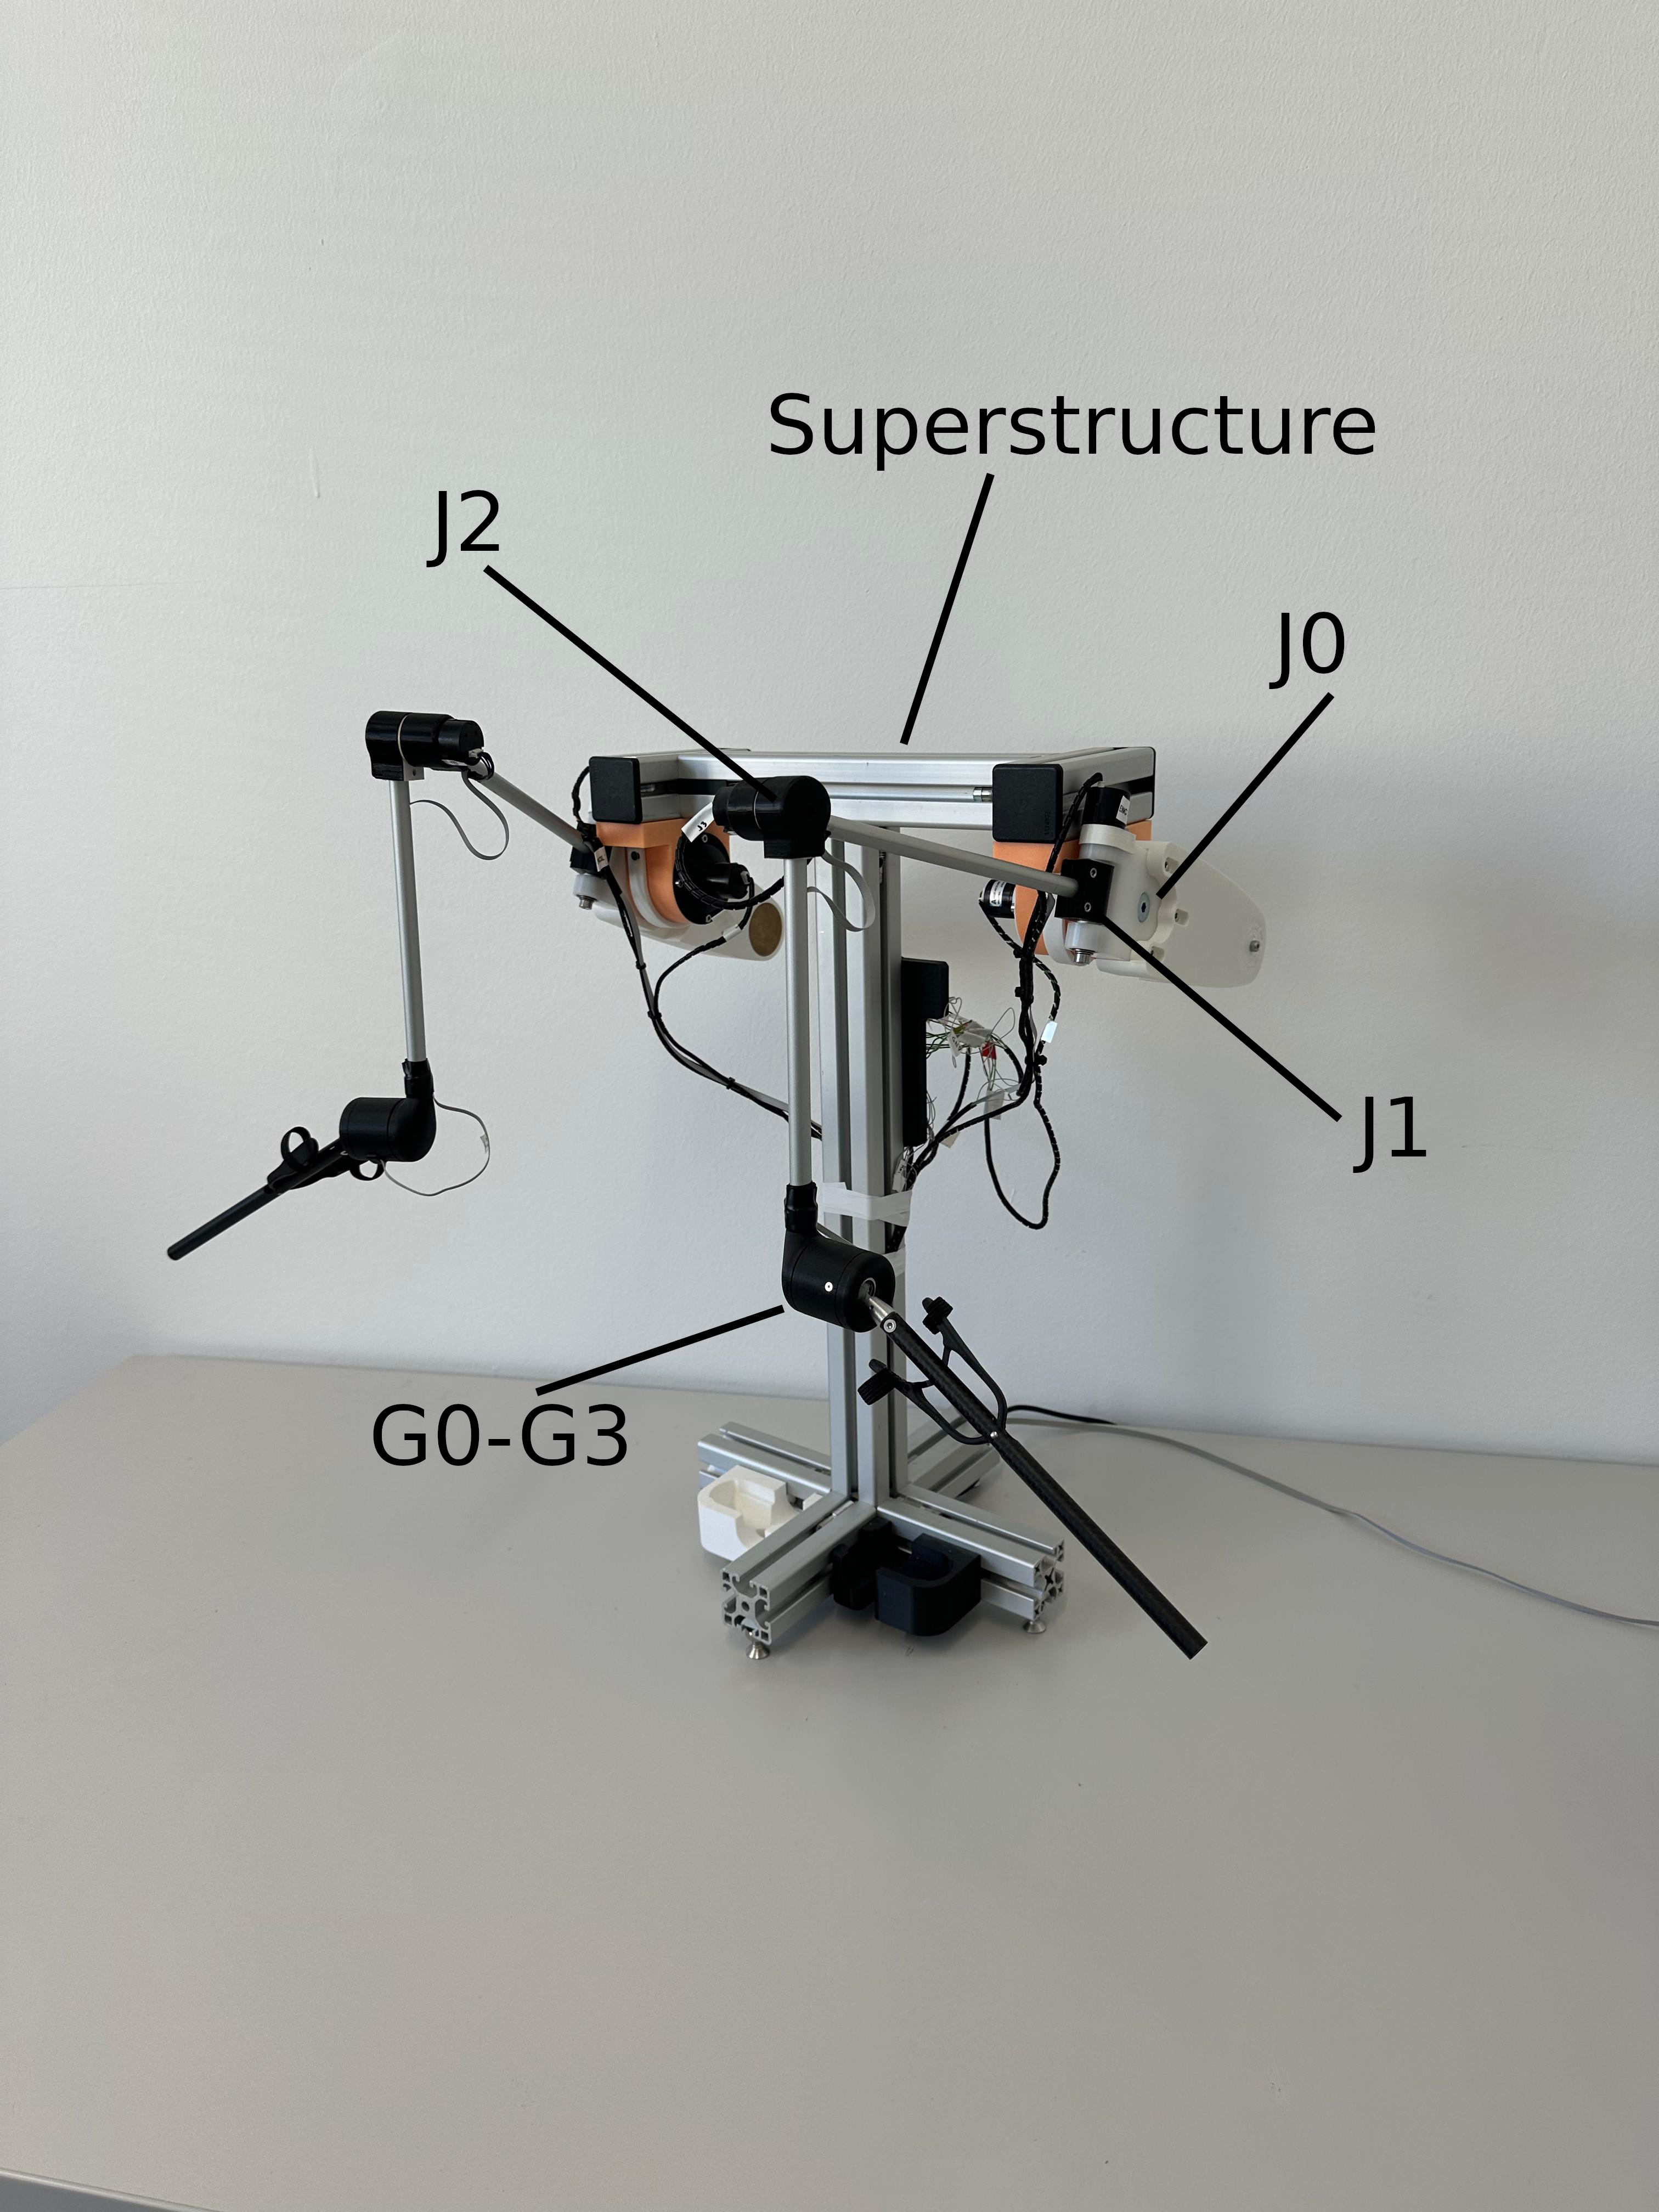
\includegraphics[width=.6\linewidth]{figures/MTMOverview.png} % Adjust width as needed
    \caption{Overview of the MTM with indicated DOFs.}
    \label{fig:mtm_dofs}
\end{figure}

\subsection{PSM Overview}

The PSM has 7 primary DOFs, classified as shown in Table~\ref{tab:psm_dofs}.


\begin{table}[H]
    \caption{PSM Joint Classification and Drive System.}
    \label{tab:psm_dofs}
    \setlength{\tabcolsep}{4pt} % Adjust this value (e.g., 2pt, 4pt) to fine-tune column spacing
    \begin{tabular}{|p{3.0cm}|l|l|p{4.5cm}|} % Changed p{} to l for left-justification where needed
    \hline
    \textbf{Joint Class} & \textbf{DOF Name} & \textbf{Drive Type} & \textbf{Positional sensing} \\
    \hline
    \multirow{3}{3.0cm}{\raggedright Overall system positioning} & Roll & \multirow{3}{*}{Brushless DC Motor} & \multirow{3}{4.5cm}{\raggedright 12-bit absolute magnetic encoders} \\
    & Pitch & & \\
    & Insertion & & \\
    \hline
    \multirow{4}{3.0cm}{\raggedright Instrument positioning} & Instrument Roll & \multirow{4}{*}{Servo Motor} & \multirow{4}{4.5cm}{\raggedright Servo feedback} \\
    & Instrument Pitch & & \\
    & Instrument Tilt & & \\
    & Instrument Grasp & & \\
    \hline
    \end{tabular}
\end{table}


An overview of the system with indications to the specific DOFs can be seen in Figure~\ref{fig:psm_overview}.

\begin{figure}[H] % Changed from [H] for better float placement
    \centering
    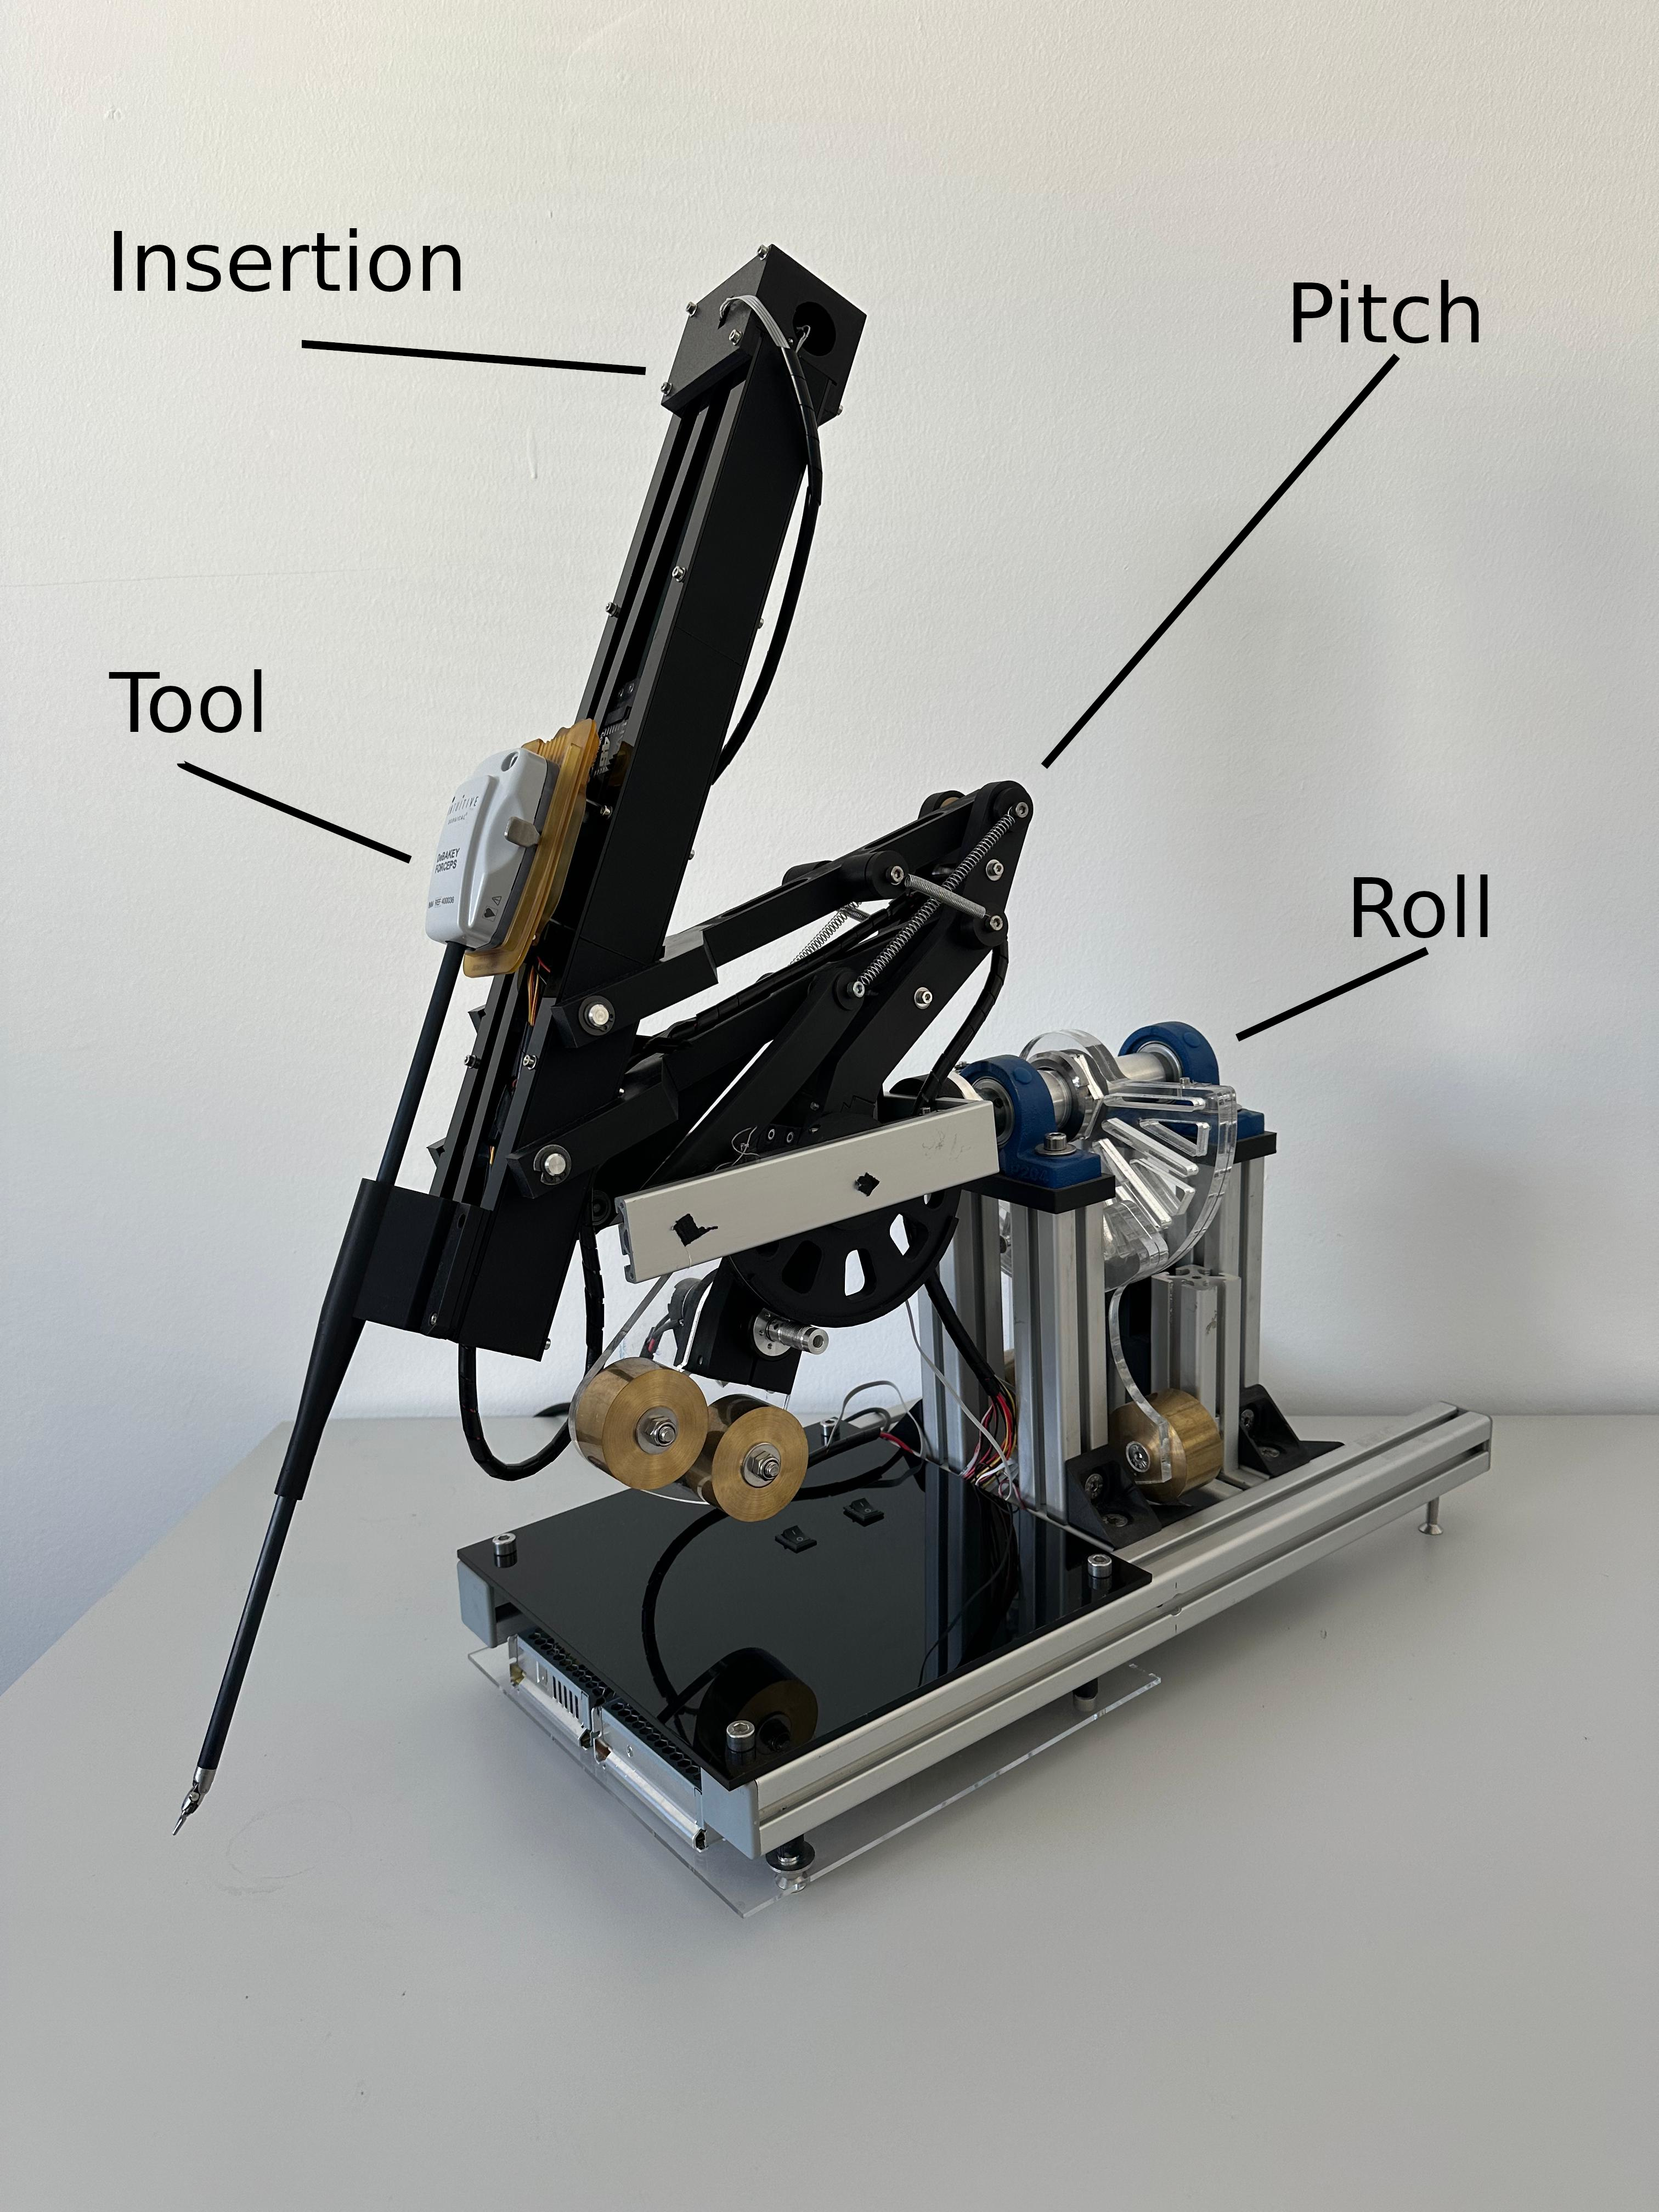
\includegraphics[width=0.6\linewidth]{figures/PSMOverview.png} 
    \caption{Overview of the PSM with indicated DOFs.}
    \label{fig:psm_overview}
\end{figure}

\section{Master Tool Manipulator Mechanical Design}

The Master Tool Manipulator (MTM) mechanical design can be separated into three subsystems, the arm (J0-J2), the gimbal (G0-G3) and the superstructure.

The arm subsystem is the primary architecture responsible for measuring the operator's position relative to the global reference frame. Three revolute joints with internal absolute magnetic encoders are coupled via rigid aluminum extrusions, allowing accurate estimation of the overall system positioning in 3D space.

The Gimbal subsystem, which is responsible for measuring the desired surgical instrument inputs, is a self-contained, 4-axis analog sensing apparatus. A 3D-printed shell contains the necessary analog sensing devices for determining the desired wrist position.

The superstructure is an aluminum extrusion structure that offsets the arm and gimbal subsystems from the table to allow space for manipulation. An overview of the design of the MTM, with indications to each subsystem, can be seen in Figure~\ref{fig:mtm_overview}.

\begin{figure}[H] % Changed from [h!] for better float placement
    \centering
    \includegraphics[width=1.0\linewidth]{figures/ArmOverview.png}
    \caption{Overview of the entire MTM system with indications to the subsystems.}
    \label{fig:mtm_overview}
\end{figure}

\subsection{Superstructure Design}

The superstructure design is relatively straightforward. With no moving parts, it is purely designed to offer a platform on which the more complicated mechanics of the MTM can be mounted.

Several pieces of 20mm x 20mm aluminum extrusion are bolted together, offering a stable and modular platform. Previously, a 3D-printed piece held an Arduino Mega at the top of the superstructure, but this was updated to hold a Teensy 4.1 on the main superstructure beam to allow for easier access and wiring. 

\subsection{Arm Joint Design}

The arm joints of the MTM feature relatively straightforward designs. The arm subsystem is rigidly coupled to the superstructure with a 3D-printed block, to which the origin of the arm's J0 joint is connected. Each joint is a simple revolute joint, directly coupled to an EAT-6012-A06 12-bit absolute magnetic encoders. These joints are then rigidly connected to each other through aluminum tubing, held in place by set screws. A detailed exploration of the J1 joint can be seen in Figure~\ref{fig:J1_detailed}. 

\begin{figure}[H] 
    \centering
    \includegraphics[width=1.00\linewidth]{figures/J1_detailed.png} 
    \caption{Detailed view of the MTM's J1 joint design (Reprinted from \cite{walder2022design} Fig 2.1)} 
    \label{fig:J1_detailed} 
\end{figure}

The design of these joints was driven by the requirement to minimize friction. Increased frictional forces in any of these joints would result in an increase in perceived force by the operator. Roller bearings were utilized to minimize these frictional forces, and system mass was also reduced to lower both gravitational and inertial forces felt by the operator. However, in an effort to completely minimize forces felt by the operator, a GCS was implemented into the J0 joint.

The GCS consists of a brass cylinder, carefully massed to offset the gravitational forces felt by the system. The exact placement and mass of this cylinder were algorithmically determined in \cite{walder2022design} A detailed view of the mechanical design of this system can be seen in Figure~\ref{fig:GCS_detailed}.

\begin{figure}[H] % Changed from [H] for better float placement
    \centering
    \includegraphics[width=1.0\linewidth]{figures/GCS_detailed.png}
    \caption{Detailed overview of the MTM's GCS design. (Reprinted from \cite{walder2022design} Fig 2.9)}
    \label{fig:GCS_detailed}
\end{figure}

\section{MTM Electrical Architecture}


\subsection{System Overview}
The MTM electrical architecture was originally based on an Arduino Mega 2560 microcontroller, which served as both the primary controller and system I/O interface. This configuration was later upgraded to a Teensy 4.1 microcontroller due to its superior performance and compatibility with ROS2 and micro-ROS frameworks.

The system incorporates multiple sensor subsystems to monitor and control the robotic arm's movements. Each DOF of the MTM is equipped with its own independent sensor for full positional sensing.

\subsection{Joint Subsystems}
Joints J0-J2 are equipped with AEAT-6012-A06 12-bit absolute magnetic encoders (resolution: 4096 counts/revolution) directly coupled to each joint axis. These encoders provide a positional accuracy of $\pm 0.088^\circ$ ($360^\circ/4096$) per joint, enabling precise positional feedback for the control system. The encoder signals are connected directly to the Teensy 4.1's digital I/O pins and are supplied 5V power directly from the Teensy 4.1.

\subsection{Gimbal Subsystem}
The wrist subsystem underwent significant design evolution. Initially, the wrist sensing utilized an MPU-6050 3-DOF IMU coupled with a Hall effect sensor for full positional sensing of the wrist subsystem \cite{Preiss2022Haptically}. However, during the course of this research, this subsystem was updated to replace the IMU with a series of three potentiometers coupled to a Hall effect sensor. G0 is measured using a Hall effect sensor on a lever arm linkage. This is then coupled to a modified FJN10K-C0 two-axis joystick potentiometer, which handles the angular sensing of G1 and G2. This joystick is coupled to the G3 potentiometer through a 3D-printed linkage. G0 used a SS495A Hall Effect Sensor, G1/G2 used a FJN10K-C0 two-axis joystick potentiometer, and G3 used a 3382H-1-103 Potentiometer.

Each of these sensors is supplied 3.3V power from the Teensy 4.1, and their resultant analog signals are sent to the Teensy 4.1's analog input pins.

\section{PSM Mechanical Design}

\subsection{Overview}
The Patient-Side Manipulator mechanical architecture is a 7-degree-of-freedom robotic system designed to replicate surgical instrument movements with high precision. The design is fundamentally inspired by the da Vinci Surgical System's remote center of motion mechanism, which maintains a fixed pivot point at the surgical incision site - a critical feature for minimally invasive surgery. The PSM can be divided into five primary subsystems., Superstructure and base, Roll axis, Pitch axis, Insertion axis, and Tool cart and end effector.

\subsection{Superstructure}
The superstructure serves as the foundational framework, constructed from 80/20 aluminum extrusion for both rigidity and modularity. The base of the superstructure also houses the necessary electronics for the control of the PSM. 

\subsection{Roll Axis}
The roll axis implements a revolute joint providing $\pm 30^\circ$ of rotation about the vertical axis. The system rotates in two roller bearings attached to the superstructure with a Commercial Off-The-Shelf bearing block. A laser-cut acrylic wheel serves as the capstan drive of the system and is clamped to the central shaft. This wheel is connected to a brushless DC motor via steel cabling, offering a 20:1 reduction in a zero-backlash setup. This shaft terminates in a forked aluminum extrusion structure, to which the pitch subsystem connects. A limit switch is attached to the superstructure to allow for zeroing of the system.

This design offered a simple way to achieve precise, zero-backlash performance in an easy-to-assemble and low-cost package. A detailed depiction of this subsystem can be seen in Figure~\ref{fig:roll_detailed}.

\begin{figure}[H] % Added placement specifier
    \centering
    \includegraphics[width=1.0\linewidth]{figures/roll_detailed.png}
    \caption{Detailed view of the mechanical design of the roll axis, highlighting the main shaft design. (Reprinted from \cite{walder2022design} Fig 2.10)}
    \label{fig:roll_detailed}
\end{figure}

To minimize forces seen by the actuator, a gravity compensation system (GCS) was applied to this joint. This GCS consisted of two adjustable brass counterweights hanging directly below the capstan drive. Their mass and placement were once again algorithmically determined by previous research conducted by Walder \cite{walder2022design}. A detailed view of the design of this GCS can be seen in Figure~\ref{fig:PSM_GCS}.

\begin{figure}[H] % Added placement specifier (requires \usepackage{float} if using [H], but [htb!] is generally better)
    \centering
    \includegraphics[width=0.75\linewidth]{figures/PSM_GCS.png}
    \caption{A detailed view of the PSM's pitch and roll GCS design. (Reprinted from \cite{walder2022design} Fig. 2.22)}
    \label{fig:PSM_GCS}
\end{figure}


\subsection{Pitch Axis}
The pitch axis replicates the Da Vinci's characteristic double parallelogram mechanism, which creates a virtual RCM distal to the joint. For ease of manufacturing, much of the PSM's pitch subsystem was designed to be 3D-printed, and for ease of assembly, many of the couplings were press-fits. This led to sagging of the mechanism and resulted in some of the linkages requiring maintenance during prolonged operation, but, overall, the linkage design was sound and maintained a remote center.

The pitch axis was coupled to the roll axis through the forked aluminum extrusion structure previously discussed in the PSM mechanical design section. Similar to the roll axis, the pitch axis was driven by a capstan drive system coupled to a brushless DC motor through steel cabling. A limit switch at the extreme limits of motion was once again used for zeroing the system, and the mechanism ultimately resulted in a $\pm 30^\circ$ range of motion. A detailed view of the pitch subsystem design can be seen in Figure~\ref{fig:pitch_detailed}.

Once again, a GCS was designed for the pitch subsystem. This design followed similar trends to the roll axis, placing a brass counterweight below the axis to reduce the force seen by the actuator. The design of this can be seen in Figure~\ref{fig:PSM_GCS}. 


\begin{figure}[H]
    \centering
    \includegraphics[width=1.0\linewidth]{figures/pitch_detailed.png}
    \caption{Detailed view of the PSM's pitch axis mechanism. (Reprinted from \cite{walder2022design} Fig 2.13)}
    \label{fig:pitch_detailed}
\end{figure}

\subsection{Insertion Axis}

The insertion axis design is relatively straightforward. A brushless DC motor coupled directly to a rack and pinion mechanism translates the rotary motion of the motor into the linear motion needed for the insertion axis. For ease of manufacturing, the majority of this mechanism was 3D-printed, and it was coupled to the pitch subsystem through a bolted connection via the end forks of the pitch linkage. For positional sensing, the carriage was coupled to an encoder through a belted connection. A detailed diagram of this subsystem can be seen in Figure~\ref{fig:insertion_detailed}.

\begin{figure}[H]
    \centering
    \includegraphics[width=1.0\linewidth]{figures/insertion_detailed.png}
    \caption{Detailed view of the PSM's insertion axis mechanism. (Reprinted from \cite{walder2022design} Fig 2.14)}
    \label{fig:insertion_detailed}
\end{figure}

\subsection{Tool Cart and End Effector}
The tool cart is responsible for driving the surgical instrument. This system uses off-the-shelf Intuitive Surgical instruments. These instruments are driven by a belted disc mechanism internal to the instrument. The tool cart houses four servo motors coupled to these discs with a spring-loaded compliance mechanism, as shown in Figure~\ref{fig:tool_cart_detailed}.

\begin{figure}[H]
    \centering
    \includegraphics[width=1.0\linewidth]{figures/tool_cart_detailed.png}
    \caption{Detailed view of the PSM's tool cart, highlighting the spring-loaded compliance mechanism. (Reprinted from \cite{walder2022design} Fig 2.15)}
    \label{fig:tool_cart_detailed}
\end{figure}



\section{PSM Electrical Architecture}

The PSM electrical architecture is based on a Teensy 4.1 as the control unit of the system. Table~\ref{tab:psm_specs} showcases each joint's associated electrical components.

\begin{table}[htb!]
    \centering
    \caption{PSM Joint Specifications} % You can adjust the caption as needed
    \label{tab:psm_specs} % You can adjust the label as needed
    % p{0.15\linewidth} for Joint column (approx 15% of text width)
    % p{0.25\linewidth} for Drive Motor (approx 25%)
    % p{0.25\linewidth} for Motor Driver (approx 25%)
    % p{0.27\linewidth} for Positional Sensing (approx 27%)
    % Total width ~0.92\linewidth, leaving some margin.
    \begin{tabular}{|p{0.15\linewidth}|p{0.25\linewidth}|p{0.25\linewidth}|p{0.27\linewidth}|}
        \hline
        \textbf{Joint} & \textbf{Drive Motor} & \textbf{Motor Driver} & \textbf{Positional Sensing} \\
        \hline
        Pitch & \multirow{3}{=}{\centering Maxon 273752 15V DC motor} & \multirow{3}{=}{\centering MD13S Cytron 13 Amp} & \multirow{3}{=}{\centering Broadcom HEDS-5540 encoder} \\
        Roll & & & \\
        Insertion & & & \\
        \hline
        Tool Roll & \multirow{4}{=}{\centering MG966r Servo} & \multirow{4}{=}{\centering None} & \multirow{4}{=}{\centering Servo Feedback} \\
        Tool Tilt & & & \\
        Tool Pitch & & & \\
        Tool Grasp & & & \\
        \hline
    \end{tabular}
\end{table}

\section{System Software Architecture}
\label{sec:software_architecture}

As noted earlier in this paper, the initial software framework was implemented in an Arduino C-based environment. While the system has since been migrated to a ROS 2 architecture, the original implementation remains relevant for context and reference.

The software was divided into two primary components: the MTM software and the PSM software. These subsystems worked in tandem to enable real-time teleoperation, with the MTM capturing user inputs and the PSM replicating movements precisely.

\subsection{MTM Software}
The MTM software was responsible for several critical functions. Sensor data was read and processed from each of the DOFs associated sensors. Data was then filtered and converted into angular measurements based on predefined system parameters. Forward kinematics were then used to calculate the end effectors position based on angular measurements from sensors. Denavit-Hartenberg (DH) parameters were used for the forward kinematic calculations. All of the associated MTM data had to be parsed into a single serial string and output to the serial monitor for later acquisition by the PSM. In addition, sensor overflow was carefully monitored and spike detection logic was implemented to catch any spikes in sensor data. All relevant data had to be packaged with start/end markers for easy access and parsing by the PSM.


\subsection{PSM Software}
The PSM software was responsible for the control and drive of the PSM based on the movements of the MTM. Upon receiving target data from the MTM through the serial monitor the data had to be parsed and processed using a custom parsing function. The target position was then extracted from this data. Each joint was controlled through a PID control function with predetermined gains. Each joint had to be homed to its 0 position and the absolute encoder 0 value was also set through a ramp-up homing sequence in which the system carefully managed joint speed as it approaches the limit of motion.
During operation limit switch state was monitored to ensure each joint was not colliding with the mechanical hard-stops. To ensure the surgical tool discs were engaged a tool catch procedure ran each servo through its complete range of motion and the PWM frequency was set to ensure that it lie outside of human range of hearing.

\section{System Controller Design}

Previous research conducted on the platform resulted in a basic controller design. Initially, a Proportional-Integral-Derivative (PID) controller was designed using the Ziegler-Nichols method. This approach involved determining the critical gain ($K_{cr}$) and periodic time ($P_{cr}$) for each joint through root locus analysis, identifying where the dominant poles intersected the imaginary axis. These values were then used with the McCormack tuning rules to calculate the initial PID constants, as presented in Table \ref{tab:pid_constants}.

\begin{table}[h!]
    \centering
    \caption{Initial PID Constants}
    \label{tab:pid_constants}
    \begin{tabular}{lccc}
        \toprule
        \textbf{Joint} & \textbf{Proportional gain ($K_p$)} & \textbf{Integral gain ($K_i$)} & \textbf{Derivative gain ($K_d$)} \\
        \midrule
        Roll & 35.0 & 50.0 & 5.0 \\
        Pitch & 60.0 & 110.0 & 15.0 \\
        Insertion & 45.0 & 800.0 & 3.8 \\
        \bottomrule
    \end{tabular}
\end{table}

However, initial trials with these derived parameters revealed significant overshoot, unacceptably long settling times, and the system frequently entered uncontrolled oscillations. As a result of these shortcomings, manual tuning of the PID coefficients was required to achieve satisfactory performance. Nevertheless, even these manually tuned PID gains still resulted in unstable oscillations, particularly at the extreme ends of the range of motion. Consequently, the system was often operated using a simple P controller with manually selected gains, leading to very poor overall system performance.


\section{System Kinematics and Coordinate Frames}

It is critical to understand the system kinematics and coordinate frames for this system. This section will illustrate the defined coordinate frame positions with the system in its respect 0 positions. 

\subsection{MTM Coordinate Frame}

As stated earlier, the MTM has 7 degrees of freedom. It is imperative to understand the coordinate frame of each of these axes. Figure \ref{fig:MTMcoords} showcases each of these axes in their zero position with their respective coordinate frames attached. A detailed view of the updated gimbal design with each of the axes in their zero position can be seen in Figure~\ref{fig:GimbalCoords}.

\begin{figure}[H]
    \centering
    \includegraphics[width=0.7\linewidth]{figures/MTMcoords.png}
    \caption{The MTM and its associated degrees of freedom shown in their zero-position with DH-coordinate frames attached (Reprinted from \cite{walder2022design} Fig 3.1)}
    \label{fig:MTMcoords}
\end{figure}

\begin{figure}[H]
    \centering
    \includegraphics[width=0.7\linewidth]{figures/Gimbalcoords.png}
    \caption{The updated gimbal and its associated degrees of freedom shown in their zero-position.  (Reprinted from \cite{Messner2025Teleoperative} Fig 2.1)}
    \label{fig:GimbalCoords}
\end{figure}

\subsection{PSM and Tool Coordinate Frame}

The PSM and its associated tool have a total of 7 degrees of freedom. Each of these degrees of freedom can be seen in their zero position in \textbf{Figure \ref{fig:PSMCoord}}.

\begin{figure}[htb!]
    \centering
    \includegraphics[width=1.0\linewidth]{figures/PSMcoord.png}
    \caption{The PSM and endowrist tool shown in their zero-position with DH-coordinate frames attached, according to the cDH convention. (Reprinted from \cite{walder2022design} Fig 3.2)}
    \label{fig:PSMCoord}
\end{figure}